\documentclass[tikz, border=12pt]{standalone}
\usepackage{newtxtext,newtxmath}
\usetikzlibrary{arrows.meta, fit, positioning, calc, backgrounds}

% ── Reuse exact palette from skills_pipeline.tex ─────────
\definecolor{steelblue}{HTML}{576fa0}
\definecolor{steelbluelight}{HTML}{a7b9d7}
\definecolor{gold}{HTML}{e3b87f}
\definecolor{goldlight}{HTML}{fadcb4}
\definecolor{rose}{HTML}{b57979}
\definecolor{roselight}{HTML}{dea3a2}
\definecolor{morandigray}{HTML}{9f9f9f}
\definecolor{morandigraylight}{HTML}{cfcece}
\definecolor{bgblue}{HTML}{e8edf5}
\definecolor{bggold}{HTML}{f5eedf}
\definecolor{bgrose}{HTML}{f0e2e2}
\definecolor{bggray}{HTML}{ececec}
\definecolor{bggreen}{HTML}{e2ede6}
\definecolor{indigo}{HTML}{6366F1}
\definecolor{indigolight}{HTML}{c7d2fe}
\definecolor{teal}{HTML}{0d9488}
\definecolor{teallight}{HTML}{99f6e4}
% new layer-specific backgrounds
\definecolor{bgindigo}{HTML}{eef0fd}
\definecolor{bgteal}{HTML}{e6f7f4}

\begin{document}
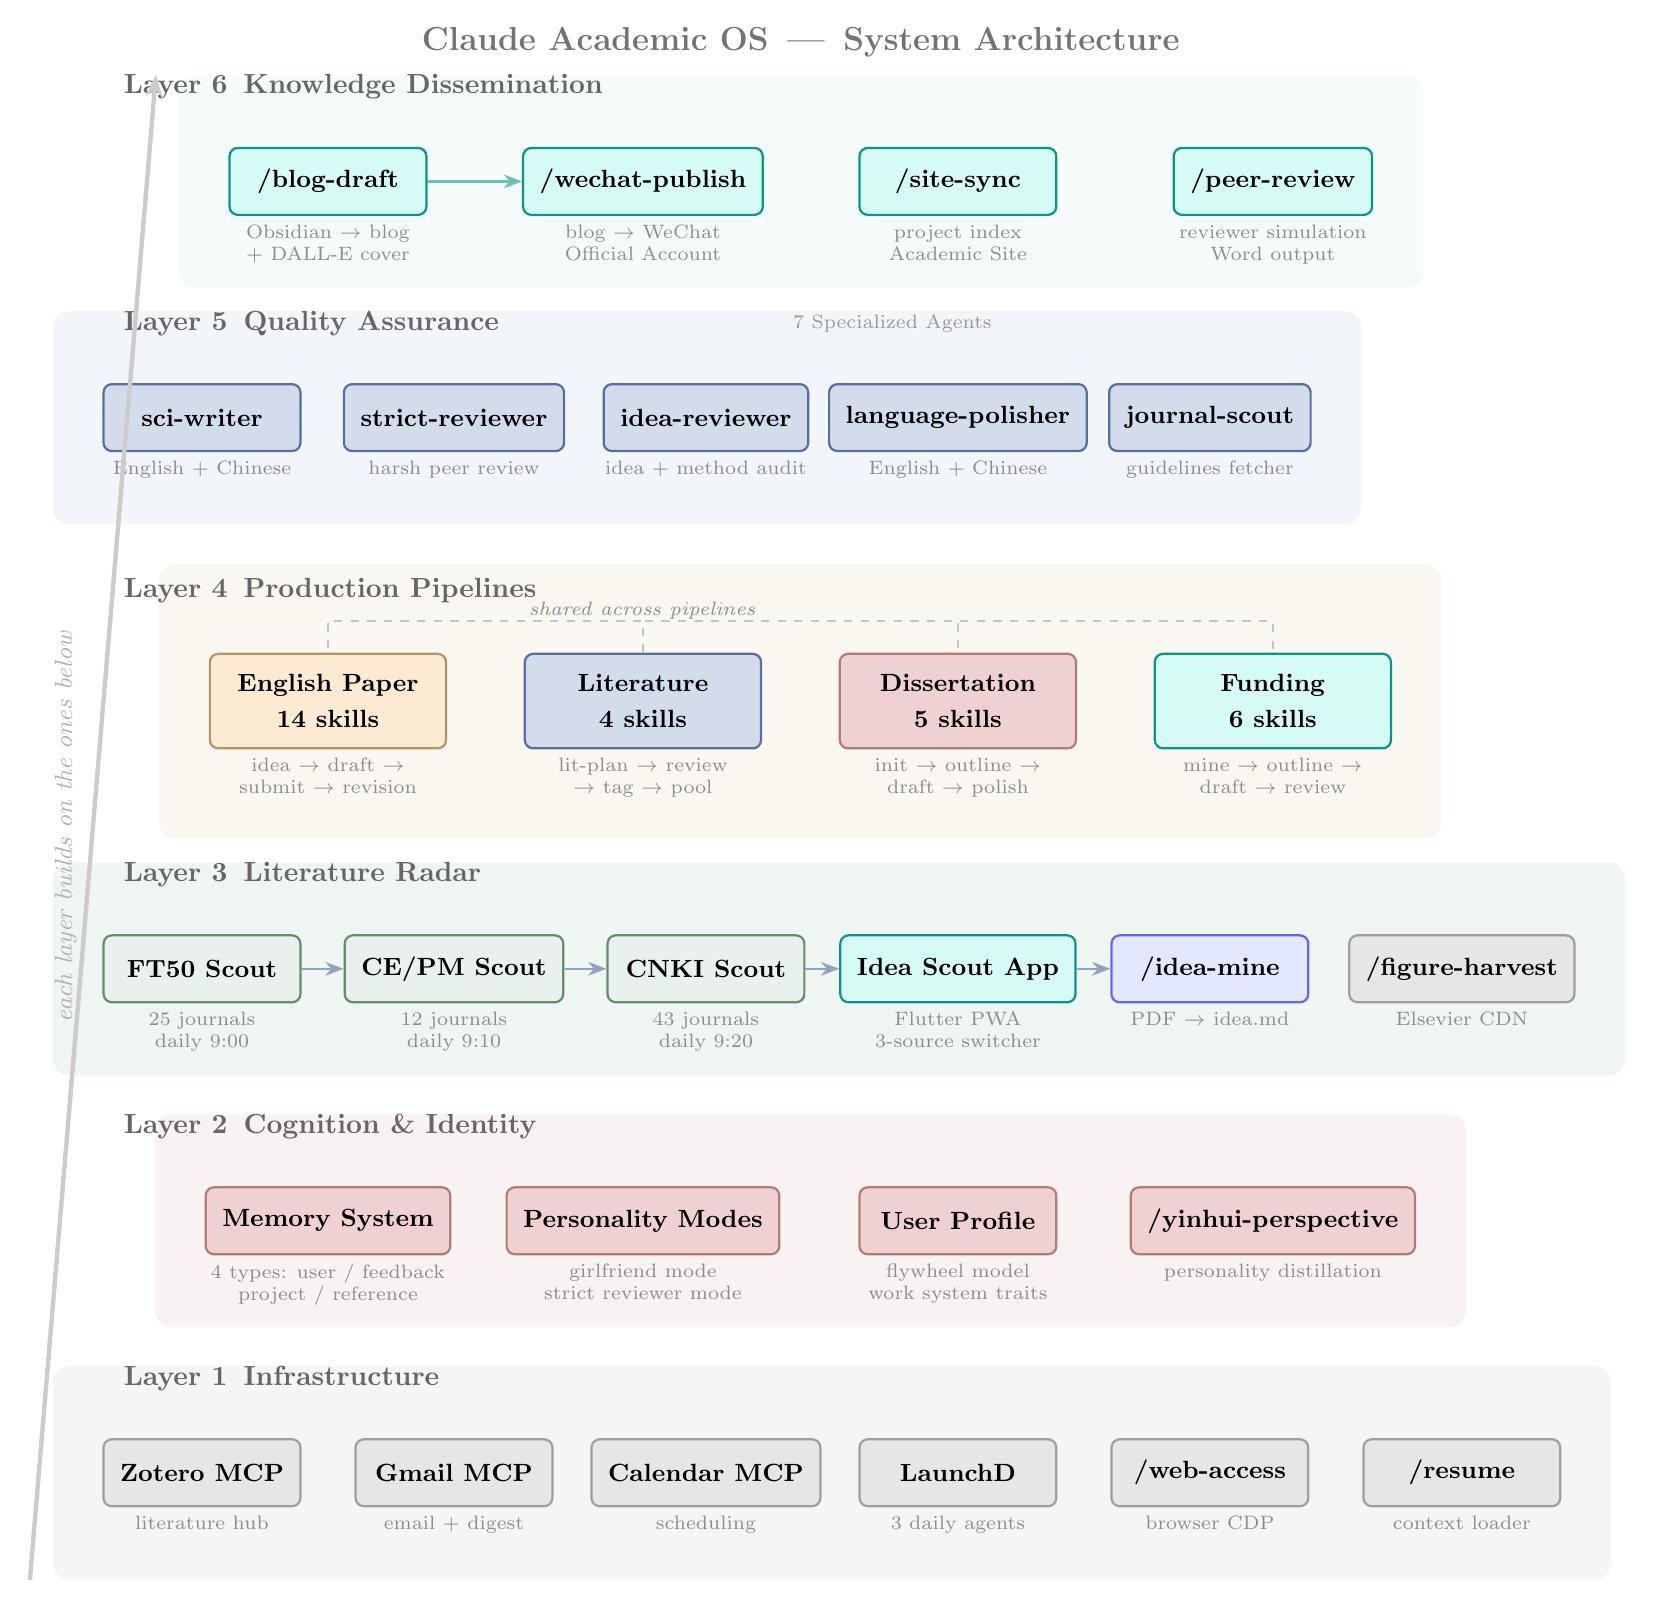
\begin{tikzpicture}[
  font=\small,
  >=Stealth,
  every node/.style={inner sep=0pt},
  % ── Same box styles as skills_pipeline.tex ────────
  skill/.style={
    draw=steelblue, thick, rectangle, rounded corners=3pt,
    fill=steelbluelight!50, align=center, inner sep=6pt,
    minimum width=2.5cm, minimum height=0.85cm,
    font=\small\bfseries,
  },
  skillgold/.style={
    draw=gold!80!black, thick, rectangle, rounded corners=3pt,
    fill=goldlight!60, align=center, inner sep=6pt,
    minimum width=2.5cm, minimum height=0.85cm,
    font=\small\bfseries,
  },
  skillrose/.style={
    draw=rose, thick, rectangle, rounded corners=3pt,
    fill=roselight!50, align=center, inner sep=6pt,
    minimum width=2.5cm, minimum height=0.85cm,
    font=\small\bfseries,
  },
  skillgray/.style={
    draw=morandigray, thick, rectangle, rounded corners=3pt,
    fill=morandigraylight!50, align=center, inner sep=6pt,
    minimum width=2.5cm, minimum height=0.85cm,
    font=\small\bfseries,
  },
  skillgreen/.style={
    draw={rgb,255:red,100;green,140;blue,110}, thick, rectangle, rounded corners=3pt,
    fill=bggreen!80, align=center, inner sep=6pt,
    minimum width=2.5cm, minimum height=0.85cm,
    font=\small\bfseries,
  },
  skillindigo/.style={
    draw=indigo, thick, rectangle, rounded corners=3pt,
    fill=indigolight!50, align=center, inner sep=6pt,
    minimum width=2.5cm, minimum height=0.85cm,
    font=\small\bfseries,
  },
  skillteal/.style={
    draw=teal, thick, rectangle, rounded corners=3pt,
    fill=teallight!40, align=center, inner sep=6pt,
    minimum width=2.5cm, minimum height=0.85cm,
    font=\small\bfseries,
  },
  % ── Pipeline box (larger, for Layer 4) ───────────
  pipebox/.style={
    draw=gold!80!black, thick, rectangle, rounded corners=3pt,
    fill=goldlight!60, align=center, inner sep=6pt,
    minimum width=3.0cm, minimum height=1.2cm,
    font=\small\bfseries,
  },
  desc/.style={font=\scriptsize\color{black!45}, align=center},
  phase/.style={font=\normalsize\bfseries, text=black!60},
  layernum/.style={font=\Large\bfseries, text=black!30},
  arr/.style={->, thick, steelblue!65},
]

%% ============================================================
%% LAYER 1 — Infrastructure (y = 0)
%% ============================================================
\node[phase, anchor=west] at (-1.0, 1.2) {Layer 1\enspace Infrastructure};

\node[skillgray] (zotero) at (0, 0) {Zotero MCP};
\node[desc, below=3pt of zotero] {literature hub};

\node[skillgray] (gmail) at (3.2, 0) {Gmail MCP};
\node[desc, below=3pt of gmail] {email + digest};

\node[skillgray] (gcal) at (6.4, 0) {Calendar MCP};
\node[desc, below=3pt of gcal] {scheduling};

\node[skillgray] (launchd) at (9.6, 0) {LaunchD};
\node[desc, below=3pt of launchd] {3 daily agents};

\node[skillgray] (webaccess) at (12.8, 0) {/web-access};
\node[desc, below=3pt of webaccess] {browser CDP};

\node[skillgray] (resume) at (16.0, 0) {/resume};
\node[desc, below=3pt of resume] {context loader};

%% ============================================================
%% LAYER 2 — Cognition & Identity (y = 3.2)
%% ============================================================
\def\Ly{3.2}
\node[phase, anchor=west] at (-1.0, \Ly + 1.2) {Layer 2\enspace Cognition \& Identity};

\node[skillrose] (memory) at (1.6, \Ly) {Memory System};
\node[desc, below=3pt of memory] {4 types: user / feedback\\project / reference};

\node[skillrose] (personality) at (5.6, \Ly) {Personality Modes};
\node[desc, below=3pt of personality] {girlfriend mode\\strict reviewer mode};

\node[skillrose] (userprofile) at (9.6, \Ly) {User Profile};
\node[desc, below=3pt of userprofile] {flywheel model\\work system traits};

\node[skillrose] (yinhui) at (13.6, \Ly) {/yinhui-perspective};
\node[desc, below=3pt of yinhui] {personality distillation};

%% ============================================================
%% LAYER 3 — Literature Radar (y = 6.4)
%% ============================================================
\def\Lz{6.4}
\node[phase, anchor=west] at (-1.0, \Lz + 1.2) {Layer 3\enspace Literature Radar};

\node[skillgreen] (ft50) at (0, \Lz) {FT50 Scout};
\node[desc, below=3pt of ft50] {25 journals\\daily 9:00};

\node[skillgreen] (cepm) at (3.2, \Lz) {CE/PM Scout};
\node[desc, below=3pt of cepm] {12 journals\\daily 9:10};

\node[skillgreen] (cnki) at (6.4, \Lz) {CNKI Scout};
\node[desc, below=3pt of cnki] {43 journals\\daily 9:20};

\node[skillteal] (app) at (9.6, \Lz) {Idea Scout App};
\node[desc, below=3pt of app] {Flutter PWA\\3-source switcher};

\node[skillindigo] (ideamine) at (12.8, \Lz) {/idea-mine};
\node[desc, below=3pt of ideamine] {PDF $\to$ idea.md};

\node[skillgray] (figharvest) at (16.0, \Lz) {/figure-harvest};
\node[desc, below=3pt of figharvest] {Elsevier CDN};

% flow arrows within radar
\draw[arr] (ft50) -- (cepm);
\draw[arr] (cepm) -- (cnki);
\draw[arr] (cnki) -- (app);
\draw[arr] (app) -- (ideamine);

%% ============================================================
%% LAYER 4 — Production Pipelines (y = 9.8)
%% ============================================================
\def\Lf{9.8}
\node[phase, anchor=west] at (-1.0, \Lf + 1.4) {Layer 4\enspace Production Pipelines};

\node[pipebox] (engpaper) at (1.6, \Lf) {\textbf{English Paper}\\[2pt]{\small 14 skills}};
\node[desc, below=3pt of engpaper] {idea $\to$ draft $\to$\\submit $\to$ revision};

\node[pipebox, draw=steelblue, fill=steelbluelight!50] (litpipe) at (5.6, \Lf) {\textbf{Literature}\\[2pt]{\small 4 skills}};
\node[desc, below=3pt of litpipe] {lit-plan $\to$ review\\$\to$ tag $\to$ pool};

\node[pipebox, draw=rose, fill=roselight!50] (diss) at (9.6, \Lf) {\textbf{Dissertation}\\[2pt]{\small 5 skills}};
\node[desc, below=3pt of diss] {init $\to$ outline $\to$\\draft $\to$ polish};

\node[pipebox, draw=teal, fill=teallight!40] (fund) at (13.6, \Lf) {\textbf{Funding}\\[2pt]{\small 6 skills}};
\node[desc, below=3pt of fund] {mine $\to$ outline $\to$\\draft $\to$ review};

% shared annotation
\draw[thick, dashed, steelblue!40] (litpipe.north) -- ++(0, 0.4) -| (engpaper.north);
\draw[thick, dashed, steelblue!40] (litpipe.north) -- ++(0, 0.4) -| (diss.north);
\draw[thick, dashed, steelblue!40] (litpipe.north) -- ++(0, 0.4) -| (fund.north);
\node[desc, anchor=south] at ([yshift=12pt]litpipe.north) {\textit{shared across pipelines}};

%% ============================================================
%% LAYER 5 — Quality Assurance (y = 13.4)
%% ============================================================
\def\Le{13.4}
\node[phase, anchor=west] at (-1.0, \Le + 1.2) {Layer 5\enspace Quality Assurance};
\node[font=\scriptsize\color{black!40}, anchor=west] at (7.5, \Le + 1.2) {7 Specialized Agents};

\node[skill] (sciwriter) at (0, \Le) {sci-writer};
\node[desc, below=3pt of sciwriter] {English + Chinese};

\node[skill] (reviewer) at (3.2, \Le) {strict-reviewer};
\node[desc, below=3pt of reviewer] {harsh peer review};

\node[skill] (ideareviewer) at (6.4, \Le) {idea-reviewer};
\node[desc, below=3pt of ideareviewer] {idea + method audit};

\node[skill] (langpolish) at (9.6, \Le) {language-polisher};
\node[desc, below=3pt of langpolish] {English + Chinese};

\node[skill] (jscout) at (12.8, \Le) {journal-scout};
\node[desc, below=3pt of jscout] {guidelines fetcher};

%% ============================================================
%% LAYER 6 — Knowledge Dissemination (y = 16.4)
%% ============================================================
\def\Ls{16.4}
\node[phase, anchor=west] at (-1.0, \Ls + 1.2) {Layer 6\enspace Knowledge Dissemination};

\node[skillteal] (blog) at (1.6, \Ls) {/blog-draft};
\node[desc, below=3pt of blog] {Obsidian $\to$ blog\\+ DALL-E cover};

\node[skillteal] (wechat) at (5.6, \Ls) {/wechat-publish};
\node[desc, below=3pt of wechat] {blog $\to$ WeChat\\Official Account};

\node[skillteal] (sitesync) at (9.6, \Ls) {/site-sync};
\node[desc, below=3pt of sitesync] {project index\\Academic Site};

\node[skillteal] (peerrev) at (13.6, \Ls) {/peer-review};
\node[desc, below=3pt of peerrev] {reviewer simulation\\Word output};

% flow arrow
\draw[arr, teal!60] (blog) -- (wechat);

%% ============================================================
%% BACKGROUND REGIONS (same style as skills_pipeline.tex)
%% ============================================================
\begin{scope}[on background layer]
  \node[fit=(zotero)(resume), inner xsep=18pt, inner ysep=26pt,
        fill=bggray!50, rounded corners=6pt] (bg1) {};
  \node[fit=(memory)(yinhui), inner xsep=18pt, inner ysep=26pt,
        fill=bgrose!45, rounded corners=6pt] (bg2) {};
  \node[fit=(ft50)(figharvest), inner xsep=18pt, inner ysep=26pt,
        fill=bggreen!55, rounded corners=6pt] (bg3) {};
  \node[fit=(engpaper)(fund), inner xsep=18pt, inner ysep=32pt,
        fill=bggold!45, rounded corners=6pt] (bg4) {};
  \node[fit=(sciwriter)(jscout), inner xsep=18pt, inner ysep=26pt,
        fill=bgblue!55, rounded corners=6pt] (bg5) {};
  \node[fit=(blog)(peerrev), inner xsep=18pt, inner ysep=26pt,
        fill=bgteal!45, rounded corners=6pt] (bg6) {};
\end{scope}

%% ============================================================
%% LEFT ARROW: "each layer builds on the ones below"
%% ============================================================
\draw[ultra thick, -{Stealth[length=8pt]}, black!20]
  ([xshift=-8pt]bg1.west |- bg1.south) -- ([xshift=-8pt]bg6.west |- bg6.north)
  node[midway, rotate=90, anchor=south, yshift=5pt,
       font=\small\itshape, text=black!30] {each layer builds on the ones below};

%% ============================================================
%% TITLE
%% ============================================================
\node[font=\large\bfseries, text=black!55, anchor=south]
  at ([yshift=6pt]bg6.north) {Claude Academic OS\enspace---\enspace System Architecture};

\end{tikzpicture}
\end{document}
